\section{Prüfung 27.09.2021}
\subsection{Echtzeit}
\subsection{a)}

\begin{figure}[H]
  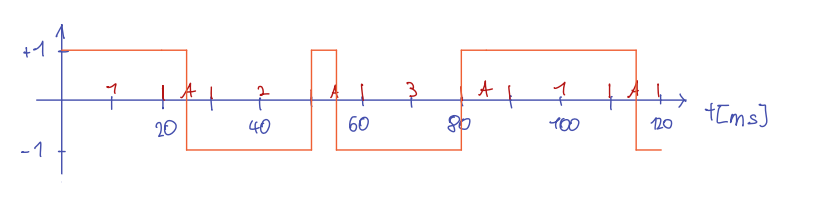
\includegraphics[width=10cm]{images/KA270921/1a.PNG}
  \centering
\end{figure}

\subsection{b)}
Handelt es sich hier um weiche, feste oder harte Echtzeit? Begründen Sie!

Es handelt sich um harte Echtzeit. Wenn angenommen wird, dass eine fehlerhafte Übertragung z.B. ein Bremsmanöver
nicht durchführen lässt, könnte es zu der Zerstörung der Maschine kommen.

\subsection{Architektur, Plattformen und Vernetzung}
\subsubsection{a)}
Unter welchen Umständen würden Sie ein Triple-Modular Redundancy (TMR) System wählen statt
eines Standby-Kontrollsystem mit Reservekontroller?

TMR wird bevorzugt wenn eine höhere Ausfallsicherheit und hohe Verfügbarkeit erfordert wird.
Wenn eine einfache Lösung gefordert ist, kann auf ein Standby-Kontrollsystem mit Reservekontroller
umgestiegen werden.

\subsubsection{b)}
Unter welchen Umständen würden Sie sich für den Einsatz eines Digitalen Signalprozessors (DSP) statt
eines ASIC entscheiden?

An ASIC is a highly specialized device constructed for one specific purpose application only, very expensive.
DSPs können für verschiedenste Signalverarbeitungs Anwendungen verwendet werden und sind deshalb flexibler wie ASICs.

\subsubsection{c)}
Warum verwendet man in eingebetteten Echtzeitsystemen oftmals Spezialhardware anstatt PCs „von
der Stange“ einzusetzen?

PCs von der Stange sind normalerweise General Purpose Operating Systems welche nicht für die spezialisierten Anwendungen
und Anforderungen von Echtzeitsystem gebaut wurden. 

\subsubsection{d)}
Unter welchen Umständen würden Sie sich für den Einsatz eines CAN-Busses anstatt eines I2C-Busses
entscheiden?

Wird eine Nachricht von mehreren Empfängern benötigt, würde man CAN bevorzugen da dieser nicht wie I2C nur an eine 
bestimmte Addresse senden kann. Mit CAN kann jeder zu jedem beliebigem Zeitpunkt Daten senden.

\subsection{Echtzeit Scheduling}
\subsubsection{a)}

\subsection{Tasksynchronisation}
Gegeben seien die drei Tasks T1, T2 und T3 wie unten dargestellt. Die Tasks werden nur einmal
abgearbeitet und enden dann. Die Semaphoren haben zu Beginn folgende initiale Werte: S1=0, S2=1, S3=0.
Gehen Sie davon aus, dass der Scheduler nicht preemptiv ist, d.h. ein Task wird solange ausgeführt bis er
durch ein wait() suspendiert wird.
\begin{figure}[H]
  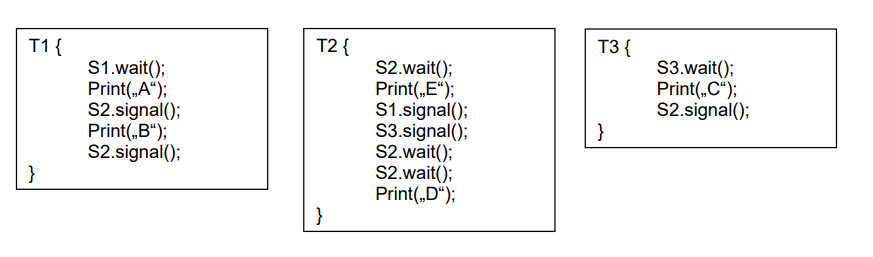
\includegraphics[width=10cm]{images/KA270921/4a.PNG}
  \centering
\end{figure}

\subsubsection{a)}
Geben Sie an in welcher Reihenfolge die Buchstaben ausgedruckt werden!

Unter der Annahme, dass T1, T2 und T3 im Round Robin verfahren gescheduled werden.

E, C, A, B, D


\subsubsection{b)}
Geben Sie die Werte der drei Semaphoren nach Ende der Abarbeitung der Tasks an!

\begin{itemize}
  \item T3: $S1 = 1$, $S2 = 1$, $S3 = 0$
  \item T1: $S1 = 0$, $S2 = 3$, $S3 = 0$
  \item T2: $S1 = 0$, $S2 = 1$, $S3 = 0$
\end{itemize}

\subsection{Spezifikationssprachen}
Zeichnen Sie einen StateChart für die Steuerung eines Scheibenwischers. Am Stellhebel können drei
Einstellungen vorgenommen werden: AUS (Scheibenwischer ausgeschaltet), LANGSAM (ein Wischvorgang
alle 30 Sekunden), SCHNELL (ein Wischvorgang alle 10 Sekunden). Dies sind die Eingabeereignisse der
Steuerung. Als Ausgabe soll die Steuerung WISCHEN zu jenen Zeitpunkten liefern wann der nächste
(einmalige) Wischvorgang ausgelöst werden soll.
Geben Sie wie bei StateCharts üblich die Namen aller Zustände an, markieren Sie Transitionen mit Eingaben
(bzw. Ereignissen) und Ausgaben, geben Sie die Startzustände an.

\begin{figure}[H]
  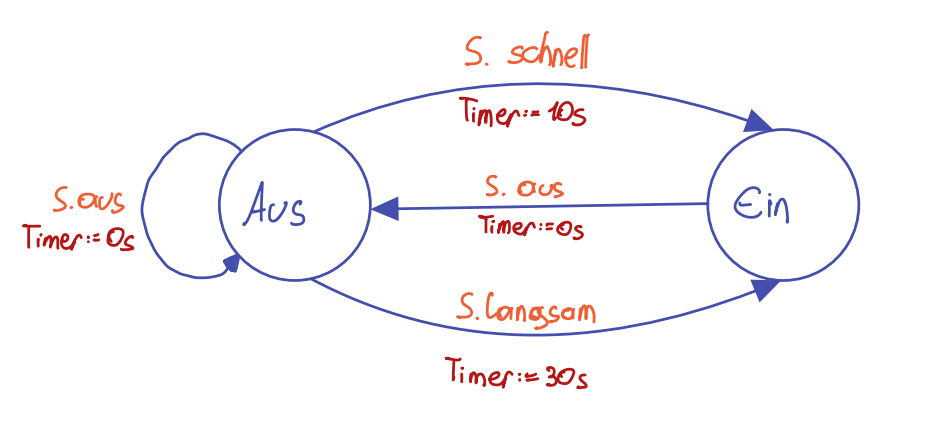
\includegraphics[width=10cm]{images/KA270921/5a.PNG}
  \centering
\end{figure}

\subsection{Speicherprogrammierbare Steuerung (SPS)}
Geben Sie zu folgendem Strukturierten Text eine Anweisungsliste und einen Kontaktplan an welche die
gleiche Funktion ausführen wie der Strukturierte Text:

\begin{lstlisting}
IF A AND NOT D THEN
  B := FALSE;
ELSE
  B := TRUE;
END_IF;
IF B OR C THEN
  E = TRUE;
ELSE
  E = FALSE;
END_IF;
\end{lstlisting}

\subsubsection{Anweisungsliste (AWL)}
Da es kein? ST NOT gibt invertieren wir die IF Abfrage zu $\neg A \lor B$, wenn dies eintritt
kann B gesetzt werden.
\begin{lstlisting}
  LDN A
  OR D
  ST B
  
  LD B
  OR C
  ST E
\end{lstlisting}

\subsubsection{Kontaktplan (KOP)}
\begin{figure}[H]
  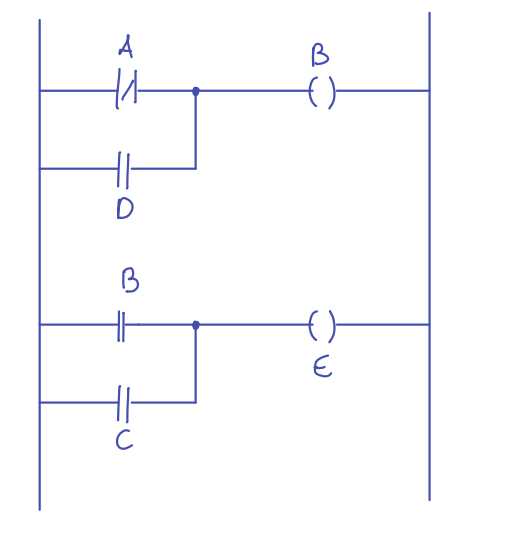
\includegraphics[width=10cm]{images/KA270921/6a.PNG}
  \centering
\end{figure}